\chapter{Experimentación}
\label{cap:experimentacion}

\section {Mapeado en entorno doméstico}
\label{cap:mapeadodomestico}

\section {Navegación con obstáculos dinámicos}
\label{cap:navegacionconobstaculos}

\section {Experimentación en la Robocup}
\label{cap:experimentacionrobocup}



{Navegacion por entornos desconocidos}

Además esta modificación nos ha permitido localizarnos en entornos desconocidos, es decir, ahora contamos con la capacidad de navegar por estancias de una casa que no tenemos en el mapa. Estas estancias se irán añadiendo al mapa de corto plazo primero y más tarde al mapa de largo plazo y el algoritmo de localización puede seguir calculando nuestra posición en los nuevos mapas.

\begin{figure}[hbtp]
  \begin{center}
    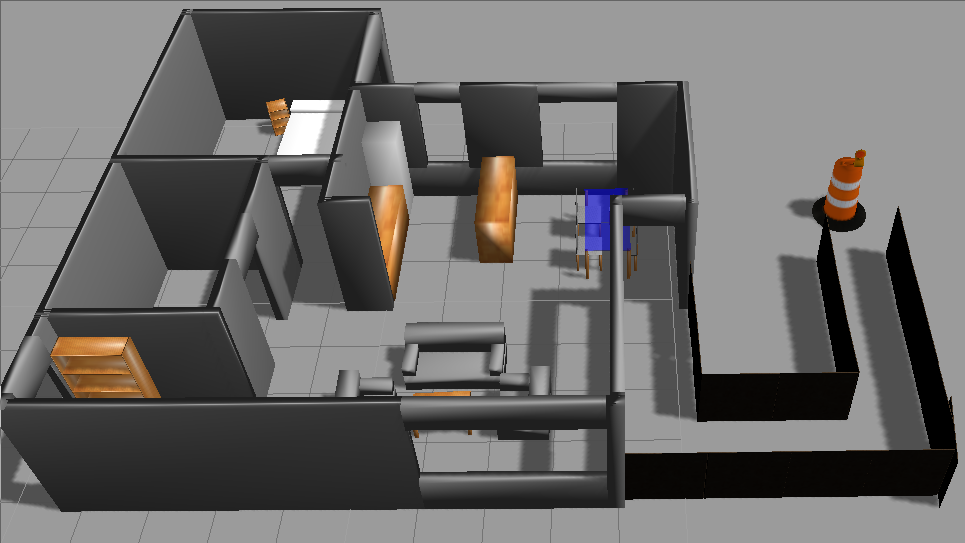
\includegraphics[width=12cm,height=7cm]{img/cap6/grannieAnne-ext}
  \end{center}
  \caption{Escenario extendido}
  \label{fig:grannieAnne-ext}
\end{figure}

\begin{figure}[hbtp]
  \begin{center}
    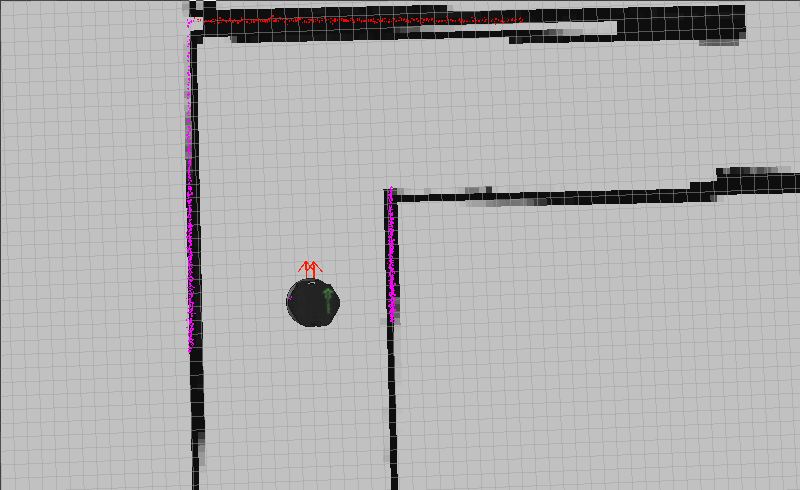
\includegraphics[width=10cm,height=6cm]{img/cap6/localization-ext}
  \end{center}
  \caption{Detalle de la localización}
  \label{fig:localization-ext}
\end{figure}


\begin{figure}[hbtp]
  \begin{center}
    \subfigure[Mapa total]{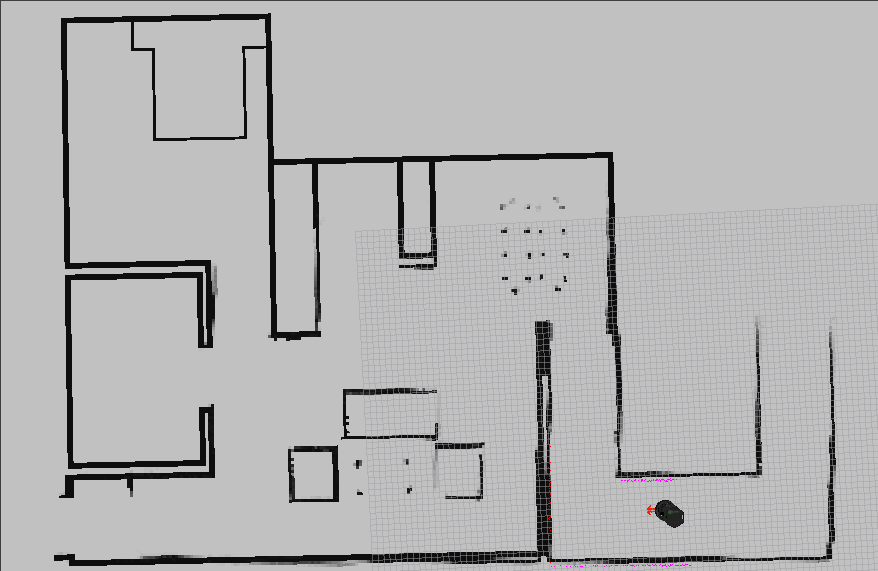
\includegraphics[width=12cm,height=7cm]{img/cap6/map-ext}}
    \subfigure[Mapa de largo plazo]{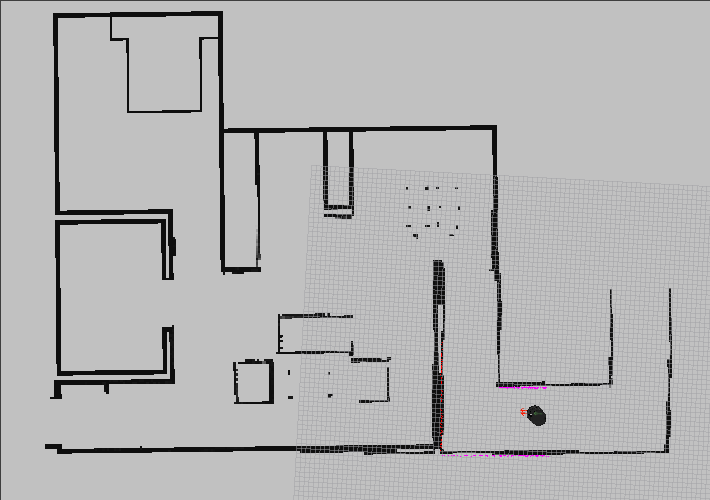
\includegraphics[width=12cm,height=7cm]{img/cap6/longmap-ext}}
    \subfigure[Mapa de corto plazo]{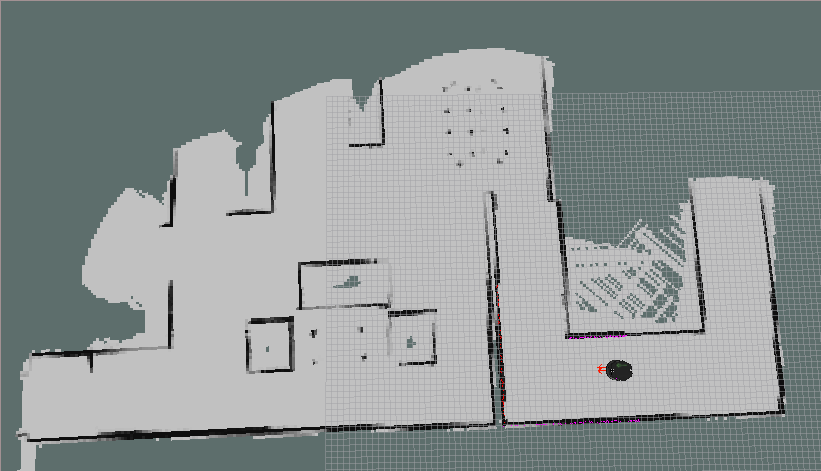
\includegraphics[width=12cm,height=7cm]{img/cap6/shortmap-ext}}
  \end{center}
  \caption{Mapas del escenario extendido}
  \label{fig:maps-ext}
\end{figure}

En la figura \ref{fig:grannieAnne-ext} vemos como el escenario ha sido extendido, añadiéndole unos pasillos a la derecha de la casa. El mapa estático usado es el mismo que el mostrado en la figura \ref{fig:mapaestatico}. Vemos como después de recorrer la parte desconocida del mapa se ha añadido al mapa de largo plazo y también al mapa total, figura \ref{fig:maps-ext}. Observamos en las flechas rojas bajo el robot que la incertidumbre en la posición del robot es mínima, figura \ref{fig:localization-ext}. 